\section{Background}

\subsection{Named Data Networking (NDN)}
Named Data Networking (NDN) \cite{zhang2014named} is a novel Internet architecture, which provides data-centric communication primitives. In NDN the communication is initiated by consumer sending the Interest packet, with the unique Name present the desired content. Any end host or router can satisfy the prefix of that name can serve for that Interest and send the Data packet back. One Interest packet can only retrieve at most one Data packet. The Name defined in the Interest packet will be used as the routing information and also presented the content of the data. Since the NDN use the name to specify what consumer wants, the Interest can be satisfied in anywhere in the Network, which isolates the data from the location information. Interest packet could be satisfied by the original data producer or by a third-party storage provider. The in-network router cache can also serve the incoming Interest packets by looking up the Name in the Content Storage inside the router. Since in NDN the name presents the content of the Data packets, the data retrieving can be done by specify the name of the data instead of individual end-to-end connection. It is more easier to share data in distributed way in NDN instead of current TCP/IP network.

NDN uses a content-based authenticity model by requiring every data packets to be signed \cite{yu2015name}, which ensures that all data packets are generated by the trusted host. For now the NDN already supports the RSA/ECDSA NDN signature to verify data source and integrity and RSA/ECDSA NDN key to encrypt/decrypt attribute private key \cite{afanasyev2016content}. They support the security requirement for the distribution data retrieving. Whatever the place data come from, the signature stays with the data and can be verified by any consumer with correct trust anchor chain.

\subsection{Attribute Based Encryption(ABE)}
Attribute-based encryption is a type of public-key encryption \cite{brucker2010attribute}. Based on the attributes, the private key can be generated for different person and ciphertext can be generated by the attributes rule. Attribute-based encryption make it possible that the user with the set of attributes which satisfy the encryption attributes policy can decrypt the ciphertext. The concept of attribute-based encryption was first proposed by Amit Sahai and Brent Waters \cite{sahai2005fuzzy} and later by Vipul Goyal, Omkant Pandey, Amit Sahai and Brent Waters\cite{goyal2006attribute}. A crucial security aspect of Attribute-Based Encryption is collusion-resistance: An adversary that holds multiple keys should only be able to access data if at least one individual key grants access. For example, assuming Alice has the key policy shown in Fig.\ref{fig:abeKey}, Alice can decrypt the content with the attribute set \{"Computer Science", "Admission committee"\}. But she cannot decrypt another ciphertext associated with attributes \{"Computer Science", "Program committee"\}.

\begin{figure}
  \centering
  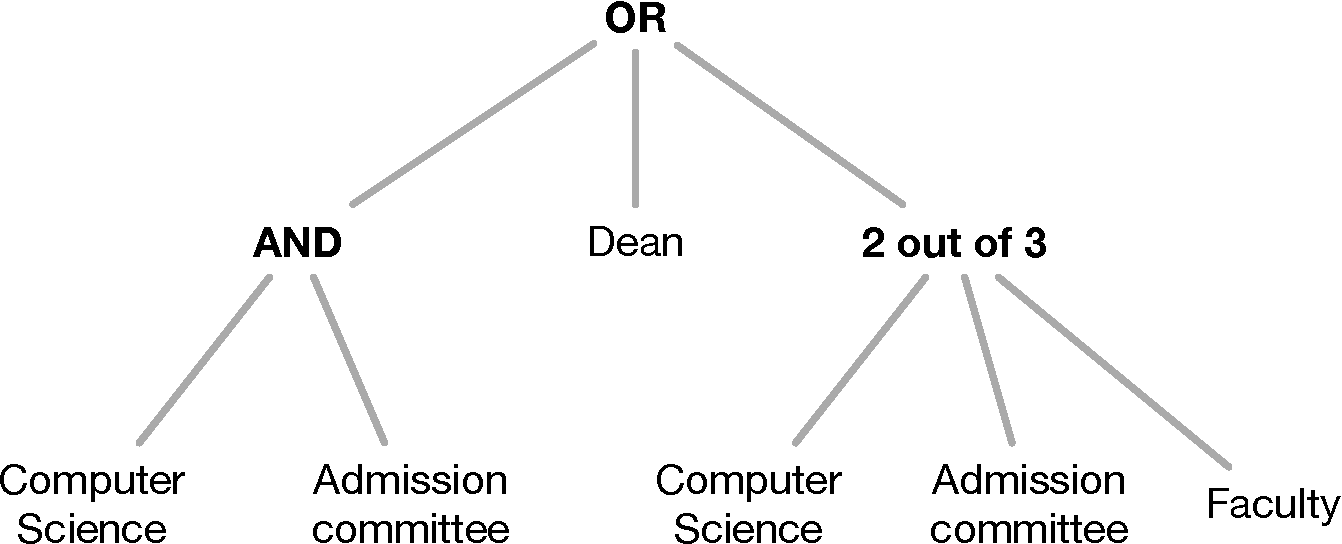
\includegraphics[width=0.45\textwidth]{Figures/ABEExample}
  \caption{Key Policy Example}
  \label{fig:abeKey}
\end{figure}

There are mainly two types of Attribute-Based Encryption schemes: Key-Policy Attribute-Based Encryption (KP-ABE)\cite{goyal2006attribute} and Ciphertext-Policy Attribute-Based Encryption (CP-ABE)\cite{bethencourt2007ciphertext}, shown in Fig.\ref{fig:KPandCPABE}. In KP-ABE, users' secret keys are generated based on an access tree that defines the privileges scope of the concerned user, and data are encrypted over a set of attribute. However, CP-ABE uses access trees to encrypt data and users' secret keys are generated over a set of attribute. In this paper the CP-ABE is applied. The producer defines the access trees to encrypt the data and registers the corresponding  name prefix. The consumer with the attributes which satisfy the privileges scope can decrypt the data. However, since the ABE can only support limited length of ciphertext, in this paper we use Advanced Encryption Standard (AES, symmetric) and Cipher Block Chaining (CBC) to encrypt/decrypt plain text, then use CPABE (asymmetric) to encrypt/decrypt AES key.

\begin{figure}
  \centering
  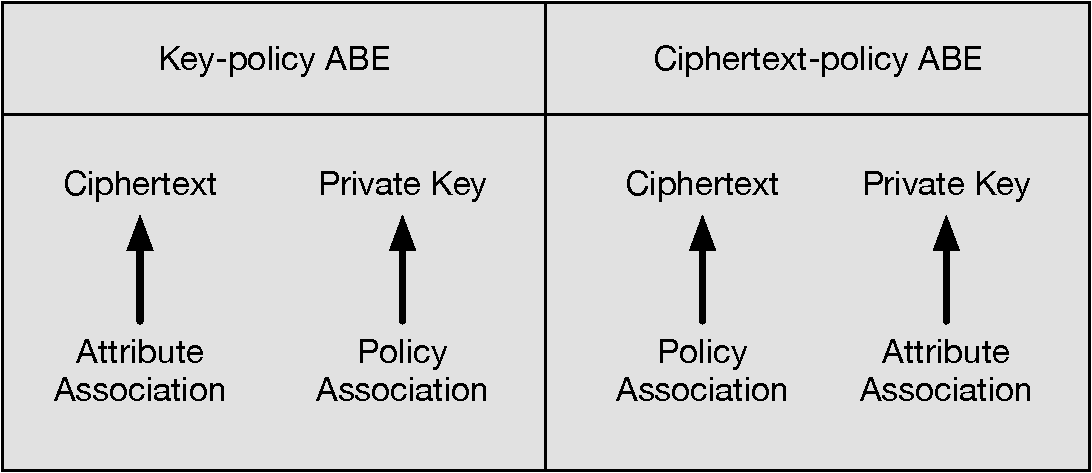
\includegraphics[width=0.45\textwidth]{Figures/KPandCPABE}
  \caption{Key Policy Example}
  \label{fig:KPandCPABE}
\end{figure}

\subsection{Advanced Encryption Standard}
Advanced Encryption Standard \cite{biham1997advanced} is a symmetric block cipher. This new symmetric key algorithm was fully open to public scrutiny and comment. In Named Based Encryption \cite{yu2015name}, the AES is also applied to encrypt the content. With Cipher Block Chaining (CBC) technique \cite{bellare1994security}, the AES can support large content ciphertext. AES is secure, low cost and easy to implement.
